%!TEX root = main.tex

\section{Index Reduction Algorithm}

\subsection{Separation of Differential and Algebraic Equations}

\begin{frame}{Index Reduction Algorithm}{Separation of Differential and Algebraic Equations}
  \vspace{-1.0em}
  \begin{columns}
    \begin{column}[c]{0.6\textwidth}
      \begin{enumerate}[<+->]
        \item Consider the \textbf{generic} \acsp{DAE} system
        \begin{equation*}
          \mF = \mA \mxp - \mb = \m{0}
        \end{equation*}
        \item \textbf{Separate} the equations with the cokernel $\mK$ and its orthogonal complement $\mN$ of $\mA$
        \begin{equation*}
          \begin{bmatrix} \mE \\ \m{0} \end{bmatrix} \mxp = \begin{bmatrix} \mg \\ \ma \end{bmatrix}
          ~~ \text{with} ~~
          \begin{array}{r@{~}c@{~}l}
            \mE &=& \mN \mA \\
            \mg &=& \mN \mb \\
            \ma &=& \mK \mb
          \end{array}
        \end{equation*}
      \end{enumerate}
      \vspace{-1.0em}
      \uncover<3->{\begin{bbox}[Cokernel Computation]
        The cokernel $\mK$ and its orthogonal complement $\mN$ of $\mA$ are calculated using matrix factorization
      \end{bbox}}
    \end{column}
    \begin{column}[c]{0.4\textwidth}
      \visible<3->{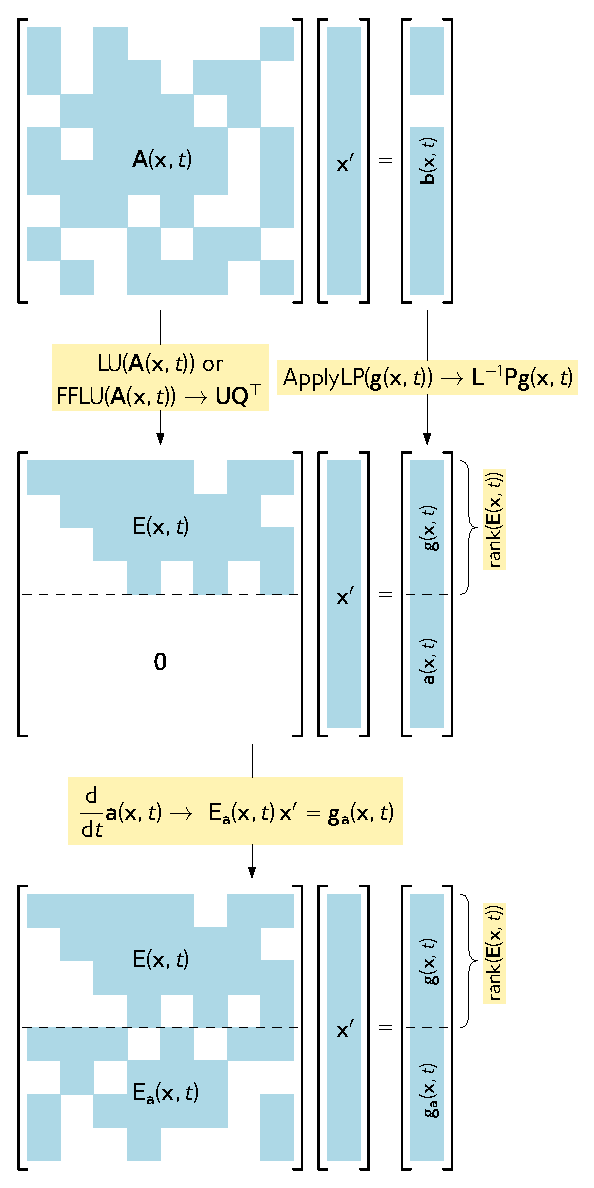
\includegraphics[width=1.0\textwidth, trim={0cm 7.35cm 0cm 0cm}, clip]{dae_visualization.eps}}
    \end{column}
  \end{columns}
\end{frame}

\subsection{Differentiation of Algebraic Equations}

\begin{frame}{Index Reduction Algorithm}{Differentiation of Algebraic Equations}
  \vspace{-1.5em}
  \begin{columns}
    \begin{column}[c]{0.6\textwidth}
      \begin{enumerate}[<+->]\setcounter{enumi}{2}
        \item Update the \textbf{invariants} as $\mh = \mh \cup \ma$
        \item \textbf{Differentiate} the algebraic equations $\ma$
        \begin{equation*}
          \dfrac{\text{d}}{\text{d}t} \ma = \mAd \mxp - \mgd
        \end{equation*}
        \item The \textbf{index reduced} system of \acsp{DAE} takes the form
        \begin{align*}
          \mF = \mA &\mxp - \mb = \m{0} ~~ \text{with} \\
          \mA = \begin{bmatrix} \mE \\ \mAd \end{bmatrix}
          ~~ &\text{and} ~~
          \mb = \begin{bmatrix} \mg \\ \mgd \end{bmatrix}
        \end{align*}
      \end{enumerate}
      \uncover<3->{\begin{bbox}[A Sequential Algorithm]
        Apply \boxednumber{1}--\boxednumber{6} repeatedly until $\mA$ is non-singular
      \end{bbox}}
    \end{column}
    \begin{column}[c]{0.4\textwidth}
      \visible<2->{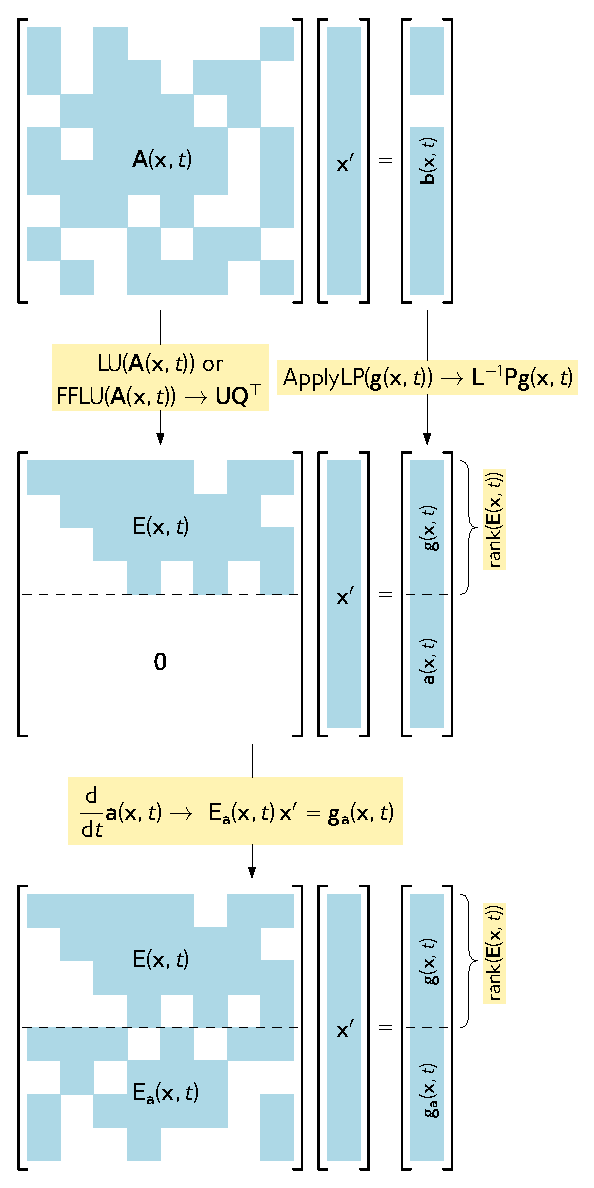
\includegraphics[width=1.0\textwidth, trim={0cm 0cm 0cm 7.35cm}, clip]{dae_visualization.eps}}
    \end{column}
  \end{columns}
\end{frame}

\begin{frame}{Index Reduction Algorithm}{Including Veiling Variables}
  \vspace{-1.0em}
  The algorithm can be extended to include \textbf{\acs{LEM}}
  \begin{itemize}
    \item veiling variables are stored in the list $\mv$
    \item equations are also function of $\mv$
    \item veiling variables add an evaluation layer to the algorithm
  \end{itemize}
  \vspace{-1.5em}\hspace{-0.025\textwidth}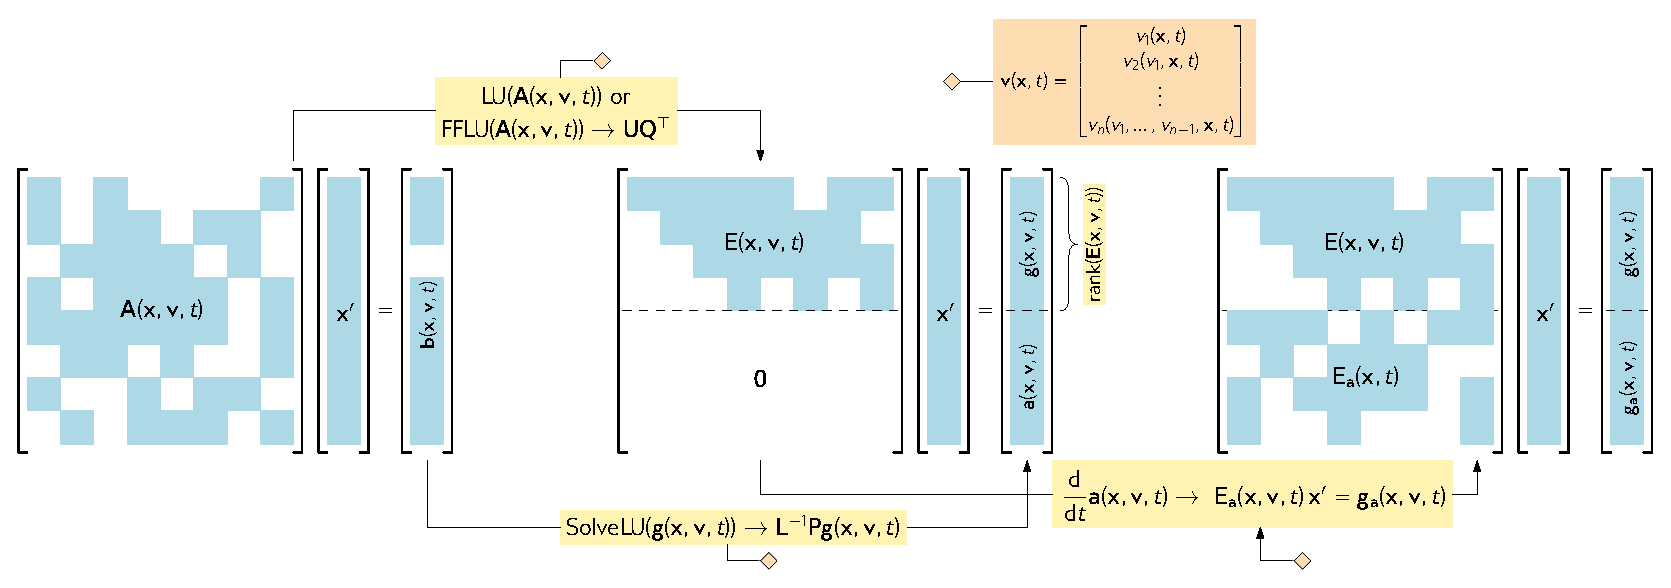
\includegraphics[width=1.05\textwidth]{dae_visualization_veil.eps}
\end{frame}

%\begin{frame}{Index Reduction Algorithm}{Algorithm Flowchart}
%  \centering
%  \begin{tikzpicture}[overlay]
%    \node at (0,0) {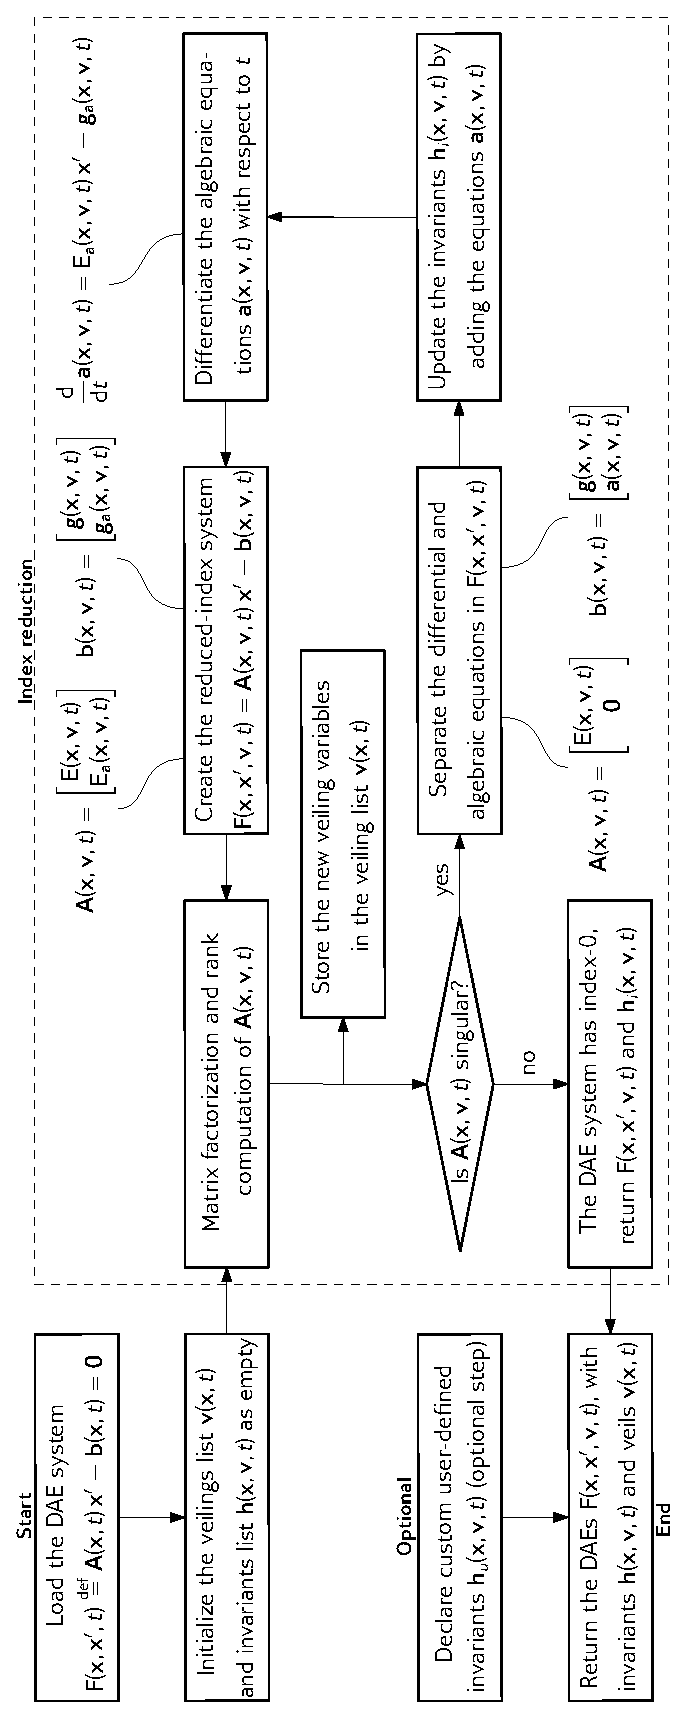
\includegraphics[angle=270, width=1.0\textwidth]{dae_flowchart_veil}};
%    \only<1>{\draw[fg_sl_color, line width=1.0pt] (-7.2,  2.9) rectangle (-3.7,  0.4);} % Initialization
%    \only<2>{\draw[fg_sl_color, line width=1.0pt] (-3.7,  2.9) rectangle ( 7.2, -2.9);} % Index Reduction
%    \only<3>{\draw[fg_sl_color, dashed, line width=1.0pt] (-7.2, -0.3) rectangle (-3.7, -1.6);} % Optional step
%    \only<4>{\draw[fg_sl_color, line width=1.0pt] (-7.2, -1.6) rectangle (-3.7, -2.9);} % Finalization
%  \end{tikzpicture}
%\end{frame}

\begin{frame}{Index Reduction Algorithm}{The Reduced \acs{DAE} System}
  \vspace{-1.0em}
  \hic{\faCanadianMapleLeaf~Now we can code-generate the reduced \acs{DAE} system!}
  \begin{itemize}[<+->]
    \item \textbf{Differential part}
    %
    \begin{equation*}
      \begin{array}{ccl}
          \m{F}(\mx, \mx^\prime, \m{v}, t) = \m{0} & \quad & \text{implicit  system class} \\
          \m{A}(\mx, \m{v}, t) \mx^\prime = \m{b}(\mx, \m{v}, t) & \quad & \text{semi-explicit system class} \\
          \mx^\prime = \m{f}(\mx, \m{v}, t) & \quad & \text{explicit system class}
      \end{array}
    \end{equation*}
    %
    \item \textbf{Invariants}
    %
    \begin{equation*}
      \m{h}(\mx, \m{v}, t) = \begin{bmatrix}
          \mhiv \\
          \mhuv
      \end{bmatrix} = \m{0} \quad \begin{array}{l}
        \text{hidden constraints} \\
        \text{\emph{optional} user-defined invariants}
        \end{array}
    \end{equation*}
    %
    \item \textbf{Veiling variables}
    %
    \begin{equation*}
        \m{v}(\mx, t) = \begin{bmatrix}
            v_{1}(\mx, t) \\
            v_{2}(v_{1}, \mx, t) \\
            \vdots \\
            v_{n}(v_{1}, \dots, v_{n-1}, \mx, t)
        \end{bmatrix}
    \end{equation*}
  \end{itemize}
\end{frame}

\subsection{Projection on Invariants}

\begin{frame}{Projection on Invariants}{Theoretical Background and Implementation}
  \vspace{-1.0em}
  \hic{\faAngleRight\hspace{-0.1em}\faAngleRight\hspace{-0.1em}\faAngleRight~Now we can integrate the system in \Matlab{}!}
  \begin{columns}
    \begin{column}[c]{0.6\textwidth}
      Projection is performed:
      \begin{itemize}
        \item during the \textbf{numerical integration}
        \item to \textbf{enforce} the solution $\mx$ onto the $\mhv$ manifold
        \item by solving the \textbf{constrained minimization} problem
          \begin{align*}
            \underset{\mx}{\text{minimize}} \quad &\dfrac{1}{2}\left(\mx - \tilde{\mx}\right)^2 \\
            \text{subject to} \quad &\mhv = \m{0}
          \end{align*}
        \end{itemize}
      \end{column}
      \begin{column}[c]{0.4\textwidth}
        \hspace{-0.2\textwidth}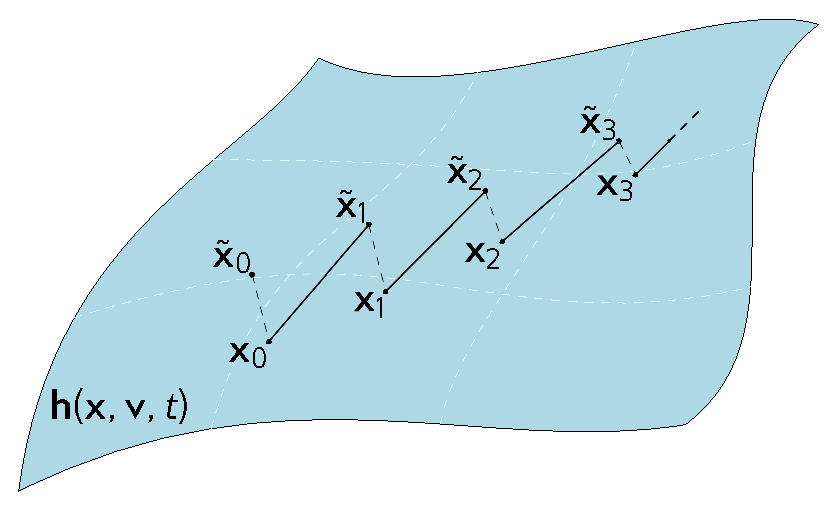
\includegraphics[width=1.2\textwidth]{projection.eps}
      \end{column}
    \end{columns}
    \vspace{1.0em}
    \hic{\large Find $\mx$ with minimal distance from $\tilde{\mx}$ that satisfies the invariants $\mhv$}
\end{frame}

%\begin{frame}{Projection on Invariants}{Theoretical Background and Implementation}
%  \begin{itemize}
%    \item The \textbf{Lagrangian} of the minimization problem is
%    \begin{equation*}
%      \mathcal{L}(\mx, \boldsymbol{\lambda}) = \frac{1}{2}\left(\mx - \tilde{\mx}\right)^2 + \boldsymbol{\lambda} \cdot \mhv
%      \quad \rightarrow \quad
%      \begin{cases}
%        \mx + \m{Jh}_\mx^\top \boldsymbol{\lambda} = \tilde{\mx} \\
%        \mhv = \m{0}
%      \end{cases}
%    \end{equation*}
%    \item The iterative method is \dots
%    \begin{equation*}
%      \begin{bmatrix}
%        \m{Jh}_{\mx} & \m{0} \\
%        \m{I}        & \m{Jh}_\mx^\top
%      \end{bmatrix}
%      \begin{bmatrix}
%        \delta\mx \\
%        \boldsymbol{\lambda}
%      \end{bmatrix} = \begin{bmatrix}
%        \tilde{\mx} - \mx \\
%        -\mhv
%      \end{bmatrix} \quad \text{where the step is} \quad \mx = \tilde{\mx} + \delta\mx
%    \end{equation*}
%    \item[] \dots derived from the \textbf{Taylor expansion}
%    \begin{equation*}
%      \begin{cases}
%        \mhv + \m{Jh}_{\mx}(\mx, \m{v}, t) \delta\mx + \textcolor{mycolor2}{\mathcal{O}\left(\| \delta\mx \|^2\right)} = \m{0} \\
%        \mx + \delta\mx + \m{Jh}_{\mx}^{\top}(\mx + \textcolor{mycolor2}{\delta \mx}, \m{v}, t) \boldsymbol{\lambda} = \tilde{\mx}
%      \end{cases}
%    \end{equation*}
%  \end{itemize}
%\end{frame}

\begin{frame}{Symbolic-Numerical Validation}{The Problem}
  \begin{columns}
    \begin{column}[c]{0.425\textwidth}
      A \textbf{particle} moving over a \textbf{torus} surface
      \begin{equation*}
        \begin{cases}
          x^{\prime}_{1} = u_{1} \\
          x^{\prime}_{2} = u_{2} \\
          x^{\prime}_{3} = u_{3} \\
          u^{\prime}_{1} = u_{3}\cos(t) - x_{3}\sin(t) - u_{2} + 2 c x_{1}\lambda \\
          u^{\prime}_{2} = u_{3}\sin(t) + x_{3}\cos(t) + u_{1} + 2 c x_{2}\lambda \\
          u^{\prime}_{3} = x_{3} + 2x_{3}\lambda \\
          \rho^2 = x_{1}^2 + x_{2}^2 + x_{3}^2 - 2r(x_{1}^2 + x_{2}^2)^{\frac{1}{2}} + r^2
        \end{cases}
      \end{equation*}
      with $c = 1 - r/(x_{1}^2 + x_{2}^2)^{\frac{1}{2}}$, $\rho = 5$, $r = 10$, and ICs $\mx_{0} = [15, 0, 0, 0, 15, -5, \lambda]^{\top}$
    \end{column}
    \begin{column}[c]{0.575\textwidth}
      \hic{\large Exact Solution}
      \begin{equation*}
        \mx_\text{exact} = \begin{bmatrix}
          x_{1} \\ x_{2} \\ x_{3}
        \end{bmatrix} = \begin{bmatrix}
          (\rho \cos(2\pi - t) + r) \cos(t) \\
          (\rho \cos(2\pi - t) + r) \sin(t) \\
          \rho \sin(2\pi - t)
        \end{bmatrix}
      \end{equation*} \\
      \centering{\includegraphics[width=0.6\textwidth, trim={17.0cm 3.5cm 2cm 2.5cm}, clip]{torus_3d_placeholder.png}}
    \end{column}
  \end{columns}
  \vspace{0.5em}
  \scriptsize{\fullcite{campbell1995constraint}}
\end{frame}

\begin{frame}{Symbolic-Numerical Validation}{Index Reduction}
  \vspace{-1.0em}
  \centering{\scriptsize\begin{tabular}{cccc}
    \multicolumn{4}{c}{\textbf{\acs{LU} Factorization}} \\
    \toprule
    \textbf{Original \acsp{DAE}} & \multicolumn{3}{c}{$\mF = 47\cf + 30\cm + 23\ca$ \quad $\mh = 0$} \\
    \midrule
    \textbf{Reduction step} & $\mE$ & $\mg$ & $\ma$ \\
    \midrule
    Index-3 \acsp{DAE} & $0$ & $39\cf + 36\cm + 13\ca$ & $7\cf + 10\cm + 6\ca$ \\
    Index-2 \acsp{DAE} & $0$ & $39\cf + 36\cm + 13\ca$ & $22\cf + 20\cm + 8\ca$ \\
    Index-1 \acsp{DAE} & $0$ & $39\cf + 36\cm + 13\ca$ & $68\cf + 72\cm + 33\ca$ \\
    Index-0 \acsp{DAE} & $388\cf + 424\cm + 180\ca$ & $79\cf + 77\cm + 26\ca$ & $0$ \\
    \midrule
    \rowcolor{mycolor5!25}
    \textbf{Reduced \acsp{DAE}} & \multicolumn{3}{c}{$\mF = 258\cf + 239\cm + 109\ca$ \quad $\mh = 97\cf + 102\cm + 47\ca$} \\
    \bottomrule \\[0.05em]
    %
    \multicolumn{4}{c}{\textbf{\acs{FFLU} Factorization}} \\
    \toprule
    \textbf{Original \acsp{DAE}} & \multicolumn{3}{c}{$\mF = 47\cf + 30\cm + 23\ca$ \quad $\mh = 0$} \\
    \midrule
    \textbf{Reduction step} & $\mE$ & $\mg$ & $\ma$ \\
    \midrule
    Index-3 \acsp{DAE} & $0$ & $39\cf + 36\cm + 13\ca$ & $7\cf + 10\cm + 6\ca$ \\
    Index-2 \acsp{DAE} & $0$ & $39\cf + 36\cm + 13\ca$ & $26\cf + 23\cm + 8\ca$ \\
    Index-1 \acsp{DAE} & $0$ & $39\cf + 36\cm + 13\ca$ & $68\cf + 72\cm + 33\ca$ \\
    Index-0 \acsp{DAE} & $388\cf + 424\cm + 180\ca$ & $79\cf + 77\cm + 26\ca$ & $0$ \\
    \midrule
    \rowcolor{mycolor2!25}
    \textbf{Reduced \acsp{DAE}} & \multicolumn{3}{c}{$\mF = 258\cf + 239\cm + 109\ca$ \quad $\mh = 101\cf + 105\cm + 47\ca$} \\
    \bottomrule \\[0.025em]
    \multicolumn{4}{c}{\small\emph{Legend}: $\cf$ = functions, $\ca$ = additions, $\cm$ = multiplications, and $\cd$ = divisions.}
    \end{tabular}}
\end{frame}

\begin{frame}{Symbolic-Numerical Validation}{Order and Error Analysis}
  \centering{\small{\input{figures/torus_order_hidden.tex}}}
\end{frame}

\begin{frame}{Symbolic-Numerical Validation}{Solution Visualization}
  \vspace{-1.0em}
  \hic{RadauIIA5 \quad $\Delta t = 0.05$\,s \quad $t \in [0, 200\pi]$\,s}
  \vspace{1.0em}
  \centering\small
  \textbf{No projection}%
  \hspace{10.0em}%
  \textbf{With projection}
  \movie[label=show1, width=0.8\textwidth, autostart, poster, showcontrols, loop]{\includegraphics[width=0.8\textwidth]{torus_3d_placeholder.png}}{movie/torus_3d.mov}
\end{frame}

% That's all Folks!